\documentclass[t]{beamer}
\usepackage[utf8]{inputenc}  % to be able to type unicode text directly
%\usepackage[french]{babel}   % french typographical conventions
\usepackage{inconsolata}     % for a nicer (e.g. non-courier) tt family font
%\usepackage{amsthm,amsmath}  % fancier mathematics
\usepackage{array} % to fine-tune tabular spacing
\usepackage{bbm} % for blackboard 1

\usepackage{graphicx}        % to include images
%\usepackage{animate}         % to include animated images
\usepackage{soul}            % for colored strikethrough
%\usepackage{bbding}          % for Checkmark and XSolidBrush
\usepackage{hyperref,url}

\colorlet{darkgreen}{black!50!green}  % used for page numbers
\definecolor{term}{rgb}{.9,.9,.9}     % used for code insets

\setlength{\parindent}{0em}
\setlength{\parskip}{1em}


% coco's macros
\def\R{\mathbf{R}}
\def\F{\mathcal{F}}
\def\x{\mathbf{x}}
\def\y{\mathbf{y}}
\def\u{\mathbf{u}}
\def\Z{\mathbf{Z}}
\def\d{\mathrm{d}}
\DeclareMathOperator*{\argmin}{arg\,min}
\DeclareMathOperator*{\argmax}{arg\,max}
\newcommand{\reference}[1] {{\scriptsize \color{gray}  #1 }}
\newcommand{\referencep}[1] {{\tiny \color{gray}  #1 }}
\newcommand{\unit}[1] {{\tiny \color{gray}  #1 }}

% disable spacing around verbatim
\usepackage{etoolbox}
\makeatletter\preto{\@verbatim}{\topsep=0pt \partopsep=0pt }\makeatother

% disable headings, set slide numbers in green
\mode<all>\setbeamertemplate{navigation symbols}{}
\defbeamertemplate*{footline}{pagecount}{\leavevmode\hfill\color{darkgreen}
   \insertframenumber{} / \inserttotalframenumber\hspace*{2ex}\vskip0pt}

%% select red color for strikethrough
\makeatletter
\newcommand\SoulColor{%
  \let\set@color\beamerorig@set@color
  \let\reset@color\beamerorig@reset@color}
\makeatother
\newcommand<>{\St}[1]{\only#2{\SoulColor\st{#1}}}
\setstcolor{red}

% make everything monospace
\renewcommand*\familydefault{\ttdefault}

\begin{document}

\begin{frame}[plain,fragile]
\LARGE
\begin{verbatim}




         ÉQUATION DE POISSON
                PAR
         RÉSEAUX DE NEURONES




\end{verbatim}
\end{frame}

% 1. contexte: intersection de trois sujets
% + objectifs du stage = (some fancy sexy words)

%SCRIPT simpois -m f/jk.png  -f one:256x128 -i f/njk.png > f/a.npy
%SCRIPT simpois -m f/njk.png -f one:256x128 -i f/njk.png > f/b.npy
%SCRIPT plambda f/a.npy f/b.npy rot_-|plambda 'x fabs 1.5 ^ x x fabs / *'|upsa 2 2 |palette -400 400 nice -l OVERLAY|plambda - 'x[2] x[1] x[0] rgb' -o f/jkpois.png
%SCRIPT blur l 2 f/jk.png|upsa 5 2|SRAND=5 plambda 'x,nn randg fabs * 0.115 <'|blur g 2|downsa v 3|qauto -p 1 - f/jkdots.png

\begin{frame}
OBJECTIF: TROUVER UNE SURFACE À PARTIR DE POINTS
================================================

\begin{tabular}{cc}
	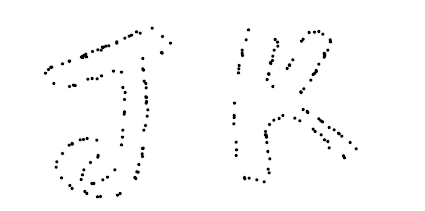
\includegraphics[width=0.46\linewidth]{f/jkdots.png} &
	
\includegraphics[width=0.46\linewidth]{f/jkdotca0.png} \\
	{\bf Entrée:} points bruités &
	{\bf Sortie:} surface lisse \\
\end{tabular}

\end{frame}

% 2. contexte: modèle de poisson pour nuages de points [ref 1]

% 3. contexte: solution par dft
% 4. contexte: solution par méthode numérique itérative multi-échelle
% 5. contexte: solution par unet-like cnn

% 6. objectif du stage: maitriser cette correspoondence, + + +

\end{document}

% 1. contexte : galleries de chuchotement
\begin{frame}
CONTEXTE: GALERIES DE CHUCHOTEMENT\\
==================================

\includegraphics[width=0.7\linewidth]{f/whisperingstpaul.jpg}

\vspace{-1.5em}
{\tiny Whispering Gallery at St. Paul's Cathedral, London}

\pause
\includegraphics[width=0.4\linewidth]{f/whispercut.jpg}
\pause
\includegraphics[width=0.25\linewidth]{f/whisper2.png}

\end{frame}


% 2. objectif du stage : conception d'une gallerie de chuchotement
% méthode: force brute pour minimiser un score de ``localisation''
% force brute = techniques modernes de ``deep learning''
\begin{frame}
OBJECTIF: CONCEPTION DE GALERIES DE CHUCHOTEMENT
================================================

\small
Est-il possible de modifier légèrement une maison afin qu'elle devienne
``chuchotable'' ?

\begin{tabular}{ll}
	\includegraphics[width=0.5\linewidth]{f/floorplan.png}&
	\includegraphics[width=0.5\linewidth]{f/floorplan3.png}\\
	{\bf Entrée:} Maison normale &
	{\bf Sortie:} Maison chuchotable\\
\end{tabular}

\vfill

\pause\color{blue}
Approche variationnelle au problème:\\
{\bf 1.} On paramètre les forme par des vecteur~$\textbf{x}\in\R^N$\\
{\bf 2.} On définit un ``score'' de chuchotabilité~$E(\textbf{x})$\\
{\bf 3.} On minimise~$E(\textbf{x})$ par force brute.

\end{frame}

% 3. cas d'école : les foyers de l'ellipse, vision corpuscle/ondes
\begin{frame}
CAS DE L'ELLIPSE\\
================

\tiny
\begin{tabular}{ll}
	\includegraphics[height=0.3\textheight]{f/youcantmiss.jpg}&
	\includegraphics[height=0.3\textheight]{f/whisper2.png}\\
	On peut chuchoter d'un foyer à l'autre... &
	...et tout au long du bord
	\\
	& \\
	& \\
	\pause
	\includegraphics[height=0.3\textheight]{f/foci.png}&
	\includegraphics[height=0.3\textheight]{f/wh3.png}\\
	Vibration localisée d'un tambour elliptique &
	Vibration au bord
	\\
\end{tabular}

\small
\color{blue}\fbox{\bf dualité billiard/tambour}

\end{frame}

% 4. vibrations globales vs. localisées (screenshots)
\begin{frame}
VIBRATIONS GLOBALES VS. LOCALISÉES
==================================

Les {\color{blue}modes normaux} d'un objet~$\Omega$ sont les fonctions propres de son
laplacien~$\Delta_\Omega$:~\fbox{$\Delta_\Omega{\color{blue}\varphi_n}=-\lambda_n{\color{blue}\varphi_n}$}

\includegraphics[width=0.25\linewidth]{f/harmonics1d.png}
\includegraphics[width=0.6\linewidth]{f/eigendumb.png}

\includegraphics[width=0.3\linewidth]{f/eigenrectangle.jpg}
\includegraphics[width=0.6\linewidth]{f/eigenell.png}

Pour des certaines formes~$\Omega$, on observe parfois des fonctions localisées
sur une partie de~$\Omega$.
\end{frame}

% 5. problème direct : calcul des modes normaux à partir de la forme
\begin{frame}
MODÉLISATION\\
============

\small 
{\bf Problème direct:} Calcul des modes normaux d'une forme~$\Omega$:\\
1. On discretise~$\Omega$ par un maillage fini ($x\in\textbf{R}^N$)\\
2. Le Laplacien discret est une matrice sym.déf.pos.~${\color{red}L}_x$\\
3. On décompose~${\color{red}L}_x={\color{blue}\Phi}_x^T{\color{darkgreen}\Sigma}_x{\color{blue}\Phi}_x$

{\bf Problème inverse:} Optimisation d'$\Omega$ pour augmenter la localisation:
\\
1. Score de localisation, e.g. $S(\varphi)=\frac
{\|\varphi\|^4_{L^2(\Omega)}}
{\|\varphi\|^4_{L^4(\Omega)}}$\\
2. On définit~$f_n:\textbf{R}^N\to\textbf{R}$ par~$f_n(x)=S(({\color{blue}\Phi}_x)_n)$\\
3. On minimise~$f_n$ par descente de gradient

\color{gray}
Les dérivées de~$f$ sont calculées par des techniques de différentiation
automatique (backpropagation) comme en deep learning.

\color{blue}
{\bf Outils:} calcul différentiel avec matrices, règle de la chaine,
modélisation d'une forme par un maillage, optimisation, stabilité numérique,
écrire un programme numérique en Python

\end{frame}

% 6. problème inverse : score de localisation, optimisation des paramètres de
% forme, règle de la chaine
\begin{frame}
	\footnotesize\color{blue}
STAGE: lecture, analyse et implémentation de ces deux articles:
===============================================================

\includegraphics[width=0.8\linewidth]{f/ref1.png}

\hrulefill

\includegraphics[width=0.6\linewidth]{f/ref2.png}

\end{frame}

\end{document}

% 7. matrices symétriques
\begin{frame}
CONTEXTE: DISSONANCE VS CONSONANCE\\
==================================

\end{frame}

% 8. plan du stage
\begin{frame}
CONTEXTE: DISSONANCE VS CONSONANCE\\
==================================

\end{frame}


%%SCRIPT cat <<END | gnuplot > f/beating.png
%%SCRIPT set term pngcairo crop size 800,400
%%SCRIPT set samples 10000
%%SCRIPT plot sin(10*x) + sin(10.5*x), 2*cos(0.25*x)
%%SCRIPT END

\begin{frame}
CONTEXTE: DISSONANCE VS CONSONANCE\\
==================================

\small
{\bf Dissonance:} phénomène de baisse fréquence (battement) dû à la
superposition de deux ondes {\em pures} de fréquence très proche.
\[
%	%e^{iFt}+e^{i(F+\epsilon)t} = e^{iFt}\cdot\left(1+e^{i\epsilon t}\right)
	\sin\left[ {\color{blue}F}t\right]
	+
	\sin\left[ {\color{blue}(F+\epsilon)}t\right]
	=
	\sin\left[ {\color{blue}(F+\tfrac\epsilon2)}t\right]
	\cdot
	2\cos\left[{\color{blue}\tfrac\epsilon2}t\right]
\]

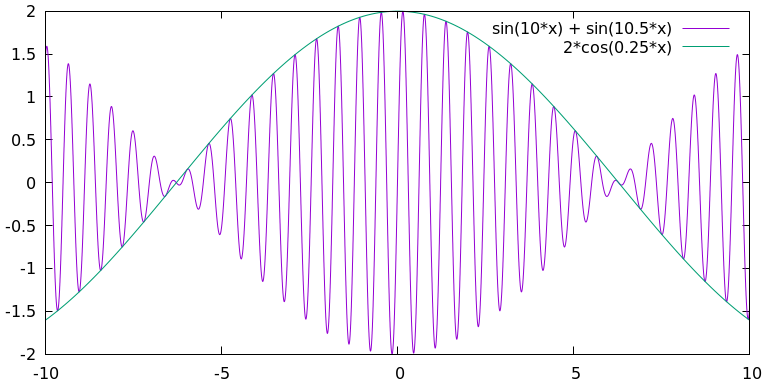
\includegraphics[width=\linewidth]{f/beating.png}
\end{frame}

%%SCRIPT cat <<END | gnuplot > f/nobeating.png
%%SCRIPT set term pngcairo crop size 800,250
%%SCRIPT set samples 10000
%%SCRIPT plot [-10:10] [-2.9:2.9] cos(10*x) + cos(20*x)
%%SCRIPT END
%%SCRIPT cat <<END | gnuplot > f/nobeating2.png
%%SCRIPT set term pngcairo crop size 800,250
%%SCRIPT set samples 10000
%%SCRIPT plot [-10:10] [-2.9:2.9] cos(10*x) + cos(20.5*x)
%%SCRIPT END

\begin{frame}
CONTEXTE: DISSONANCE VS CONSONANCE\\
==================================

\small
Le battement n'apparaît jamais pour fréquences bien éloignées.

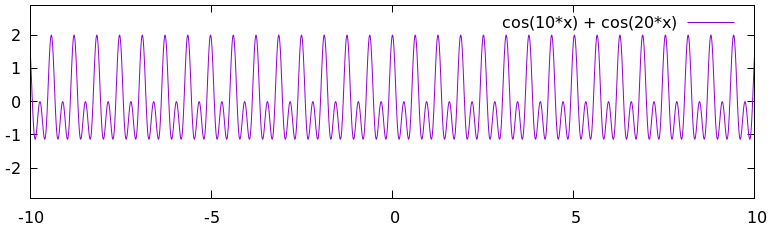
\includegraphics[width=\linewidth]{f/nobeating.png}

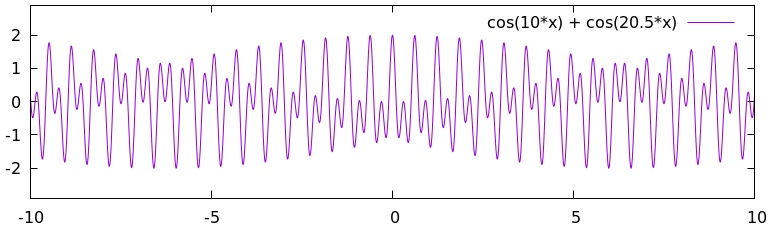
\includegraphics[width=\linewidth]{f/nobeating2.png}
\end{frame}


\begin{frame}
CONTEXTE: DISSONANCE VS CONSONANCE\\
==================================

\small
Le son des {\bf instruments traditionnels} est une %n'est pas une onde pure, mais une
somme d'ondes pures de fréquences multiples entiers de la fondamentale
\[
	s_{\color{blue}F}(t)=
	a_1\sin\left[{\color{blue} F}t\right] +
	a_2\sin\left[{\color{blue}2F}t\right] +
	a_3\sin\left[{\color{blue}3F}t\right] +
	a_4\sin\left[{\color{blue}4F}t\right] +
	\cdots
\]
%Avec les instruments musicaux traditionnels, on entend aussi du battement sur
%d'autres intervalles (ex. ceux proches à un multiple entier, comme C4--C5\#).
\only<1>{\includegraphics[width=.7\linewidth]{f/spectrograms.png}}
\only<2>{
	\[
		s_{\color{blue}(2+\epsilon)F}(t)=
		a_1\sin\left[{\color{blue} (2+\epsilon)F}t\right] +
		a_2\sin\left[{\color{blue}(4+2\epsilon)F}t\right] +
		a_3\sin\left[{\color{blue}(6+3\epsilon)F}t\right] +\cdots
	\]
	\vfill
	Ainsi, quand on joue C4+C5\# avec le piano on entend de la dissonance
	puisque les partiels sont presque bien alignés.
}

\end{frame}


\begin{frame}
CONTEXTE: DISSONANCE VS CONSONANCE\\
==================================

\small
Le {\bf gamelan}, un instrument sacré d'Indonésie avec des sons fortement
inharmoniques (les partiels ne sont pas du tout multiples entiers de la
fondamentale).

\includegraphics[width=.8\linewidth]{f/gamelan.jpg}

\end{frame}


\begin{frame}
OBJECTIF DU STAGE\\
=================

\pause
Résoudre le problème d'algèbre linéaire suivant:

Soit~$B\in\mathcal{M}_{m,n}(\mathbf{R})$ et~$\Sigma\in\mathbf{R}^n_+$
avec~$m>n$, il faut trouver~$W\in\mathbf{R}^m_+$ tel qu'il existe~$U\in
O_n(\mathbf{R})$ qui satisfait
\[
	B^\top\mathrm{diag}\left(W\right)B = U^\top\mathrm{diag}\left(\Sigma\right)U
\]
Autrement dit, il faut trouver~$W\in\mathbf{R}^m$ tel que
\[
	\mathrm{sp}_{\mathbf{R}}\left(
		B^\top\mathrm{diag}\left(W\right)B
	\right)
	=\Sigma
\]

\pause\small
{\bf Interprétation:}\\
$B=$ topologie d'un maillage\\
$W=$ poids sur les liens du maillage (forme/rigidité)\\
$\Sigma=$ spectre de vibration ($\sigma_1=$fondamentale, $\sigma_i=$partiels)\\
$U_i=$ modes de vibration
\end{frame}



\begin{frame}
OBJECTIF DU STAGE\\
=================

Construire un instrument de percussion qui produit un son de cette forme:
\[
	s_{\color{blue}F}(t)=
	\sin\left[{\color{blue} F}t\right] +
	\sin\left[{\color{blue}(2+\epsilon)F}t\right] +
	\sin\left[{\color{blue}(3+\epsilon)F}t\right] +
	\sin\left[{\color{blue}(4+\epsilon)F}t\right] +
	\cdots
\]
Ainsi, les octaves~$s_{\color{blue}F}$ et~$s_{\color{blue}2F}$ produites par
cet instrument seront fortement dissonantes.

\vfill
Problème inverse de modélisation de formes: comment trouver une forme qui a un
spectre de vibration donnée?
\end{frame}


\begin{frame}
PROBLÈME DIRECT (FACILE)\\
========================

{\bf Question:}
Étant donné la forme~$\Omega$ d'un objet, quel est son spectre de
vibration~$\Sigma$?

{\bf Réponse:}\\
1. Construire la matrice {\color{blue}$L= B^\top W_\Omega B$}\\
2. Appeler la fonction {\color{blue}scipy.sparse.linalg.eigs(L)}

\setlength{\tabcolsep}{0pt}
\begin{tabular}{ccccccccccc}
	\includegraphics[width=0.093\linewidth]{f/marsmooth.png} &
	\includegraphics[width=0.093\linewidth]{f/marbords.png} &
	\includegraphics[width=0.093\linewidth]{f/marimba_v01.png} &
	\includegraphics[width=0.093\linewidth]{f/marimba_v02.png} &
	\includegraphics[width=0.093\linewidth]{f/marimba_v03.png} &
	\includegraphics[width=0.093\linewidth]{f/marimba_v04.png} &
	\includegraphics[width=0.093\linewidth]{f/marimba_v05.png} &
	\includegraphics[width=0.093\linewidth]{f/marimba_v06.png} &
	\includegraphics[width=0.093\linewidth]{f/marimba_v07.png} &
	\includegraphics[width=0.093\linewidth]{f/marimba_v08.png} &
	\includegraphics[width=0.093\linewidth]{f/marimba_v09.png} \\
	$1\!\!1_\Omega$  & $W$ &
	$u_1$ &
	$u_2$ &
	$u_3$ &
	$u_4$ &
	$u_5$ &
	$u_6$ &
	$u_7$ &
	$u_8$ &
	$u_9$
\end{tabular}
\end{frame}

\begin{frame}
PROBLÈME INVERSE (DIFFICILE)\\
============================

{\bf Question:}
Étant donné un spectre de vibration~$\Sigma$, comment trouver un objet~$\Omega$
tel que son spectre de vibration soit~$\Sigma$?

\pause

{\bf Réponse (force brute):}
Minimiser la fonction
\[
	E(W)=\left\|
	\mathrm{sp}_\mathbf{R}\left(B^\top WB\right)
	-\Sigma
	\right\|^2
\]

\pause
{\bf Petit problème technique:}
La fonction {\color{blue}eigs} n'est pas ``différentiable'' (on ne peut pas faire backtracking).

\pause
{\bf Vrai objectif du stage:}
Une implémentation ``différentiable'' de la fonction {\color{blue}eigs} qui
sert à calculer~$\mathrm{sp}_\R(A)$.

\end{frame}



\end{document}


% vim:sw=2 ts=2 spell spelllang=fr:
